\section{Clustering: warm-up}
To warm-up, we consider the classical problem of clustering nodes distributed
in $\mathbb{R}^{2}$. To do that, we generate 100 nodes per cluster distributed according to
structures colloquially known as \textit{two-moons}, \textit{two-circles}, \textit{three-circles},
and \textit{worms}.
Figure~\ref{fig:clusters} depicts the results of learning the
clusters structures using the proposed algorithm denoted as \textit{Spectral Graph Learning} (\textsf{SGL}).
As we can note, \textsf{SGL} is able to perfectly distinguish the cluster membership
of all the datapoints for all datasets. Additionally, Figure~\ref{fig:twomoon_trend}
depicts the convergence trend of the terms in the objective function for the
\textit{two-moons} structure.

\begin{figure}[!htb]
    \centering
    \begin{subfigure}[b]{0.23\textwidth}
        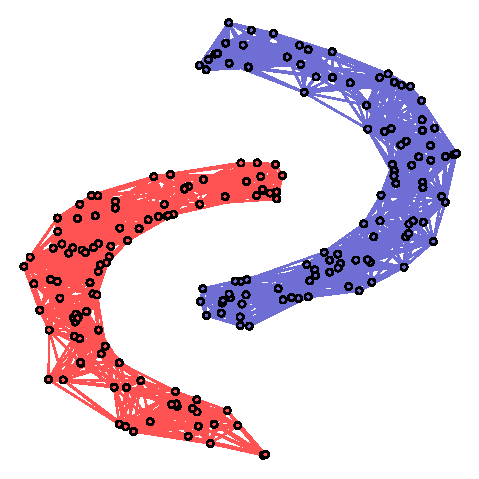
\includegraphics[width=\textwidth]{clusters/twomoon.eps}
        \caption{\textit{two-moons}.}
    \end{subfigure}
    ~ %add desired spacing between images, e. g. ~, \quad, \qquad, \hfill etc.
      %(or a blank line to force the subfigure onto a new line)
    \begin{subfigure}[b]{0.23\textwidth}
        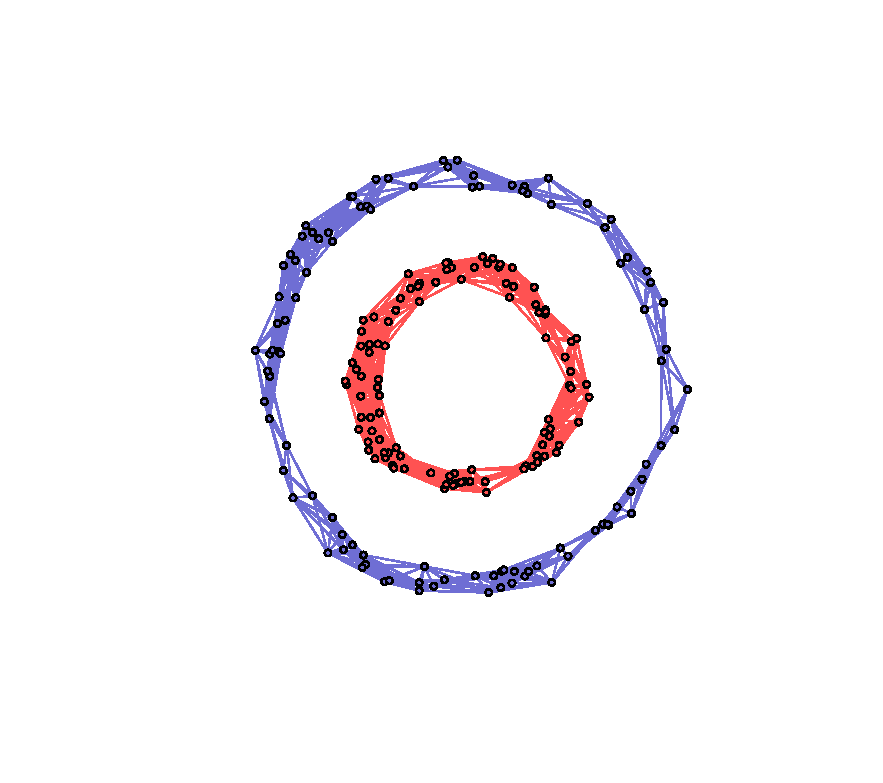
\includegraphics[width=\textwidth]{clusters/circles2.eps}
        \caption{\textit{two circles}.}
    \end{subfigure}
    ~
    \begin{subfigure}[b]{0.23\textwidth}
        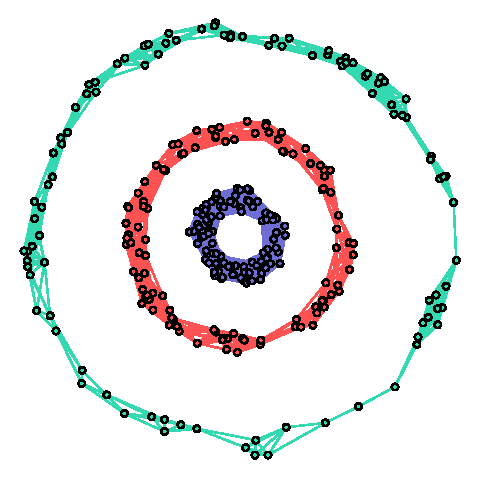
\includegraphics[width=\textwidth]{clusters/circles3.eps}
        \caption{\textit{three circles}.}
    \end{subfigure}
    \begin{subfigure}[b]{0.23\textwidth}
        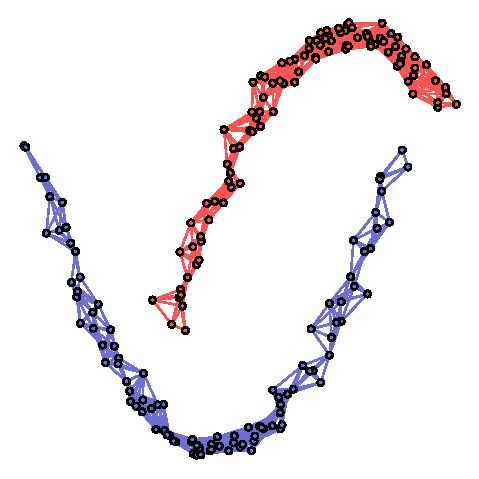
\includegraphics[width=\textwidth]{clusters/worms.eps}
        \caption{\textit{worms}.}
    \end{subfigure}
    \caption{Clustering results learned by the \textsf{SGL} algorithm for synthethic datasets.}
    \label{fig:clusters}
\end{figure}

\begin{figure}[!htb]
  \centering
  \includegraphics[width=.7\textwidth]{clusters/twomoon_trend.eps}
  \caption{Convergence trend of the \textsf{SGL} algorithm for the \textit{twomoon} dataset.}
  \label{fig:twomoon_trend}
\end{figure}
